\chapter{Evaluating dark matter signals}

\textbf{Disclaimer: All data provided is still a work in progress and may be subject to change before the final version.}

The main goal of the thesis is to investigate if certain dark matter signals can be detected after the high luminosity upgrade. One immediate worry is that the background will be large in comparison to the signal, making the signal undetectable. 

The signal models are given in \appendixref{cha:datasets} along with the background models. The different models were discussed in part in \subsectionref{sec:tb:subsec:eft} and some more in this chapter.

This thesis focus on using a luminosity at 1000 fb$^{-1}$ and a center of mass energy at 14 TeV. The reco data is created using a pile-up rate, $\obs{\mu} = 140$ as expected during phase II.

Each of these has been evaluated in different signal regions and the detectability has been evaluated using a statistical P-value. This process has been performed at different pile-up values. 

\newpage
\section{Signal to background ratio}
\subsection{Selection criteria}
For different purposes different selection criteria or regions are used. These are a set of criteria specified to enhance the area of interest. For instance, if simulating a specific signal one wants to find as many ways as possible to diminish the background. This so that when searching experimentally, the signal will be easier to detect.

These can be quite general cuts, there are only some things to take into consideration. 
\begin{itemize}
\item If experimental, what limitations are set by the detectors? Are there some criteria already?
\item If simulated, is there some criteria set in the generator?
\item Are there criteria which must be set since there is to much uncertainty in the data? or a large effect of pile up?
\end{itemize}


\subsection{Verifying background data} 	
To verify that the background data was correct it was compared with Ref. \citep{ATLAS-CONF-2012-147} in which the center of mass energy is 8 TeV and the luminosity is 10 fb$^{-1}$. Since the luminosity is not 1000 $^{-1}$ as used in this thesis the expected values from the paper scaled up with a factor 100 to be comparable. 

Somewhat unexpectedly a center of mass energy at 8 TeV required the cross-sections to be a factor 4 lower than the cross-sections at 14 TeV. \textbf{How do I reference the cross-section?}

The signal regions used in the article were the following:
\begin{table}[h]
\begin{center}
\begin{tabular}{l}
\hline
Selection Criteria \\ \hline
Jet veto, require no more than 2 jets with $p_T > 30 GeV$ and $|\eta| < 4.5$ \\
Lepton veto, no electron or muon \\
Leading jet with $|\eta| < 2.0$ and $\Delta \phi (jet, E_T^{Miss})>0.5$ (second-leading jet) \\ \hline
\end{tabular}
\begin{tabular}{l l l l l l}
signal region & SR3p & SR4p \\ \hline
minimum leading jet p$_T$ (GeV) & 350 & 500 \\
minimum E$^{Miss}_T$ (GeV) & 350 & 500 \\ \hline
\end{tabular}
\label{tab:oldsr}
\caption{The signal regions from Ref. \citep{ATLAS-CONF-2012-147}.}
\end{center}
\end{table}

The article had in total four signal regions, unfortunately since the simulated events used in this thesis are filtered before the analysis only the two highest regions are comparable. This can be seen in \subsectionref{Verifying background data} in \tableref{tab:Compare1}.

\subsection{Weight}
A weight is used to normalize different types of data so that they can be compared. In thesis the following is used:
\begin{equation}
weight=\frac{\Lagr \sigma}{N_{Raw}}
\end{equation}
where $N_{Raw}$ is number of events expected at the luminosity that was set to create the data, compared to $\Lagr$ which is the luminosity at which the data is compared and $\sigma$ is the cross-section.

\subsection{Figure of merit}
To be able to evaluate different signal regions and different signal models, a figure of merit p is used. The value p is the probability for an assumed hypothesis to be correct, thus a good signal region will yield a low value. The assumed hypothesis is that the background and its fluctuations is measured over the signal plus background.

Assuming the expected number of background events are B $\pm \sigma_B$ where $\sigma_B$ is the quadratic sum of the statistical error from Monte Carlo, the statistical error from the control region (\abbrCR) and the systematic errors. The expected number of signals is S, assumed without fluctuation. 

If no uncertainty in B or S is assumed, then the number of expected events, N, in the signal region should follow a Poisson distribution as such:
\begin{equation}
\text{P(N|S+B)}=\frac{e^{-(S+B)}(S+B)^N}{N!}
\end{equation} 

However since there is an uncertainty in the background, the probability distribution P(N|S+B) must be convoluted with a Gaussian function:
\begin{equation}
 \text{G(N$_B$|B,$\sigma_B$)}=\frac{1}{\sigma_B \sqrt{2 \pi}} e^{-\frac{(N_B-B)^2}{2\sigma_B^2}}
\end{equation}
where N$_B$ is the expected number of background events. The convolution is done using N$_B$ as N resulting in the total probability density function:
\begin{align}
\text{F(N|S+B},\sigma_B) &= \text{P(N|S+N$_B$)$\ast$G(N$_B$|B,$\sigma_B$)}= \notag \\
&=\int\limits_{-\infty}^{\infty}P(N|N_B - (S+B))G(N_B|B,\sigma_B) dN_B
\end{align}
This leads to the probability of the signal plus background fluctuation to B events being obtained by summing the probability function from N=0 to N=B.
\begin{equation}
p = \sum\limits_{i=0}^{B} \int\limits_{-\infty}^{\infty} \text{P(i|N$_B - $(S+B))G(N$_B$|B,$\sigma_B$)} dN_B
\end{equation}

In this thesis, two different models of the error in the background $\sigma_B$ are used.   
Both models are based on Ref. \citep{ATLAS-CONF-2012-147}. As described in the beginning of this subsection the error is calculated as:
\begin{equation*}
\sigma_B = \text{Statistical error from \abbrMC} \oplus \text{Statistical error in \abbrCR} \oplus \text{Systematic error}
\end{equation*}

\begin{itemize}
\item The statistical error from \abbrMC has been neglected since there is no way of estimating it for the used data.
\item The statistical error from background \abbrCR has been assumed to decrease with the increased luminosity, $\frac{30}{380} \frac{\sqrt{L_{old}}}{\sqrt{L_{new}}}$
\item The systematic error has been given two different values, from the article:\\ $\frac{30}{380}$ or fixed at 0.02.
\item All this results the total error being used as either, 0.0793411 or 0.0215018. 
\end{itemize}

\subsection{D5 operators}\label{sec:signal:subsec:d5}
As described in the introduction \subsectionref{sec:tb:subsec:eft}, one of the signals is modelled using the D5 operator. In this thesis two different scenarios were used, one at a dark matter mass of 50 GeV and one at 400 GeV.

Each of these models are modelled with a mass suppression scale, denoted M*, which is strongly correlated to the cross-section of the process.

One property which is of interest is to calculate how large M* can be so that the signal is still detectable over the background processes. Theses results are given in \subsectionref{sec:res:subsec:m*}.

\subsection{Light vector mediator models}
As described in the introduction \subsectionref{sec:tb:subsec:eft}, the other signal model is a vector mediator model. In this thesis these signals have two different width scenarios and a number of different mediator mass scenarios. In addition to this there are, as with the D5 operator two different dark matter mass scenarios.

\textbf{What is width?}

The models which are detectable are given in \subsectionref{sec:res:subsec:Mm}.
 
\newpage
\section{Other selection criteria}
\subsection{Criteria}
To be able to compare signal results to previous papers new signal regions were devised. It was also discovered that the requirement of no electrons was to harsh for the signal models. Because of this new signal criteria were devised.

\begin{table}[h]
\begin{center}
\begin{tabular}{l}
\hline
Selection Criteria \\ \hline
Jet veto, require no more than 2 jets with $p_T > 30 GeV$ and $|\eta| < 4.5$ \\
Lepton veto, no electron or muon. \\
The electron veto is defined: $\Delta R (jet^{lead},electron^{lead})\geq 0.4$ and \\
$electron^{lead} P_T>20 GeV$ removed.\\
Leading jet with $|\eta| < 2.0$ and $\Delta \phi (jet, E_T^{Miss})>0.5$ (second-leading jet) \\ 
\end{tabular}
\begin{tabular}{l l l l l l}
\hline
signal region & SR1 & SR1p & SR2 & SR3 & SR4 \\ \hline
minimum leading jet p$_T$ (GeV) & 350 &500& 600 & 800 & 1000 \\
minimum E$^{Miss}_T$ (GeV) & 350&500 & 600 & 800 & 1000 \\ \hline
signal region & SRa &  & SRb & SRc & SRd \\ \hline
minimum leading jet p$_T$ (GeV) & 350 & & 350 & 350 & 350 \\
minimum E$^{Miss}_T$ (GeV) & 350 & & 600 & 800 & 1000 \\ \hline
\end{tabular}
\label{tab:newsr}
\caption{The new signal regions}
\end{center}
\end{table}

\subsection{Verifying background data}
To make sure that the altered electron veto still produces results comparable with \citep{ATLAS-CONF-2012-147} a comparison was made again. This can be seen in \subsectionref{Verifying background data} in \tableref{tab:newcomp}.

\section{Mitigating the effect of the high luminosity}
As discussed in \subsectionref{chap:vali:sec:dis:subsec:smearindep} the effect of pile-up should be minimal in the high energy regions which are of interest in this thesis. 

Mention that the effect is on a trigger level, that the lowest SR will be lost.

Even though this was envisioned as the primary focus of the thesis, it was shown that the effect of pile-up is minute for these high signal regions. Thus the focus was shifted to perform a more in-depth mono-jet analysis of different DM signal models.
\newpage
\section{Results}\label{chap:sig:sec:res}
\subsection{Verifying background data}\label{Verifying background data}
In \tableref{tab:Compare1} a comparison has been made. It can be seen that the simulated events and expected events coincide on all accounts apart from W$\rightarrow\tau\nu$, W$\rightarrow\mu\nu$ and thus the total as well. \textbf{This can be explained by better separation of $\mu$,$\tau$ and missing energy.} 
Tau can not be reconstructed as jets in the code, they can in reality!

Here used truth data as to not be effected by pile-up.

\begin{table}[ht]
\begin{center}
\begin{tabular}{|l|l|l|l|l|}
\hline
Process & SR3p & Expected SR3p & SR4p & Expected SR4p \\ \hline
Z$\rightarrow\nu\nu$ & 140298 & 152000 & 25250.3 & 27000 \\
W$\rightarrow\tau\nu$ & 40700.8 & 37000 & 5861.74 & 3900 \\
W$\rightarrow e\nu$ & 11229 & 11200 & 1506.58 & 1600 \\
W$\rightarrow\mu\nu$ & 13727.1 & 15800 & 1872.32 & 4200 \\ \hline
Total background & 205955 & 218000 & 34491 & 36700 \\ \hline
\end{tabular}
\caption{Comparison of the simulated and expected events from \citep{ATLAS-CONF-2012-147} with $\Lagr=1000$fb$^{-1}$, cross-sections corresponding to $\sqrt{s}=8$TeV and using the same electron veto.}
\label{tab:Compare1}
\end{center}
\end{table}

\begin{table}[ht]
\begin{center}
\begin{tabular}{|l|l|l|l|l|}
\hline
Process & SR1  & Expected SR1 & SR1p & Expected SR1p  \\ \hline
Z$\rightarrow\nu\nu$ & 147009 & 152000 & 26734 & 27000 \\
W$\rightarrow\tau\nu$ & 44727.7 & 37000 & 6543.82 & 3900 \\
W$\rightarrow e\nu$ & 17964 & 11200 & 2470.46 & 1600 \\
W$\rightarrow\mu\nu$ & 14285.7 & 15800 & 1971.87 & 4200 \\ \hline
Total background & 223986 & 218000 & 37720.2 & 36700 \\ \hline
\end{tabular}
\caption{Comparison of the simulated and expected events from \citep{ATLAS-CONF-2012-147} with $\Lagr=1000$fb$^{-1}$, cross-sections corresponding to $\sqrt{s}=8$TeV and using a modified electron veto.}
\label{tab:newcomp}
\end{center}
\end{table}


\subsection{Events}
Give a table with the number of events for signals and background in all signal regions both truth and reco.

The below is only for truth, must create new code to write it for reco.


Have a table with the number of signal and bkg ground events for the different SR where the signal then is given at M* 1 GeV for a good comparison.

Same tables as above but at reco.

%\renewcommand{\arraystretch}{1.0} %Change back
%\renewcommand{\arraystretch}{1.5} %Change height of tabel
\begin{landscape}
\begin{table}[ht]
\begin{center}
\begin{tabular}{|l|l|l|l|l|l|l|l|}
\hline
Process & SRa/SR1  & SRb & SR2 & SRc & SR3 & SRd & SR4 \\ \hline
D5 mDm=50 $Q_{cut}=200$ & 50410.4 & 434.012 & 0 & 0 & 0 & 0 & 0 \\
M*=1TeV $Q_{cut}=400$ & 53242.1 & 10018.1 & 4934.73 & 159.539 & 0 & 22.0054 & 0 \\
$Q_{cut}=600$ & 26210.6 & 25958.1 & 25284.7 & 12767.2 & 10749.7 & 5199.47 & 4391.35 \\ \hline
Total signal & 129863 & 36410.1 & 30219.4 & 12926.8 & 10749.7 & 5221.48 & 4391.35 \\ \hline

Z$\rightarrow\nu\nu$ & 604479 & 58613.9 & 42656.5 & 11383.4 & 8423.89 & 2842.85 & 2110.55 \\
W$\rightarrow\tau\nu$ & 154140 & 10678.5 & 7807.06 & 1788.16 & 1307.89 & 385.861 & 295.124 \\
W$\rightarrow e\nu$ & 61771.6 & 3961.35 & 2890.39 & 653.918 & 485.485 & 152.221 & 109.887 \\
W$\rightarrow\mu\nu$ & 49114.3 & 3051.61 & 2357.17 & 498.995 & 379.201 & 108.086 & 90.9721 \\ \hline
Total background & 869505 & 76305.4 & 55711.2 & 14324.5 & 10596.5 & 3489.02 & 2606.54 \\ \hline
\end{tabular}
\caption{Signal and background events for truth data in the signal regions.}
\label{tab:srtruth1}
\end{center}
\vspace*{5px}
\begin{center}
\begin{tabular}{|l|l|l|l|l|l|l|l|}
\hline
Process & SRa/SR1 & SRb & SR2 & SRc & SR3 & SRd & SR4 \\ \hline
D5 mDm=50 $Q_{cut}=200$ & 41968.9 & 564.215 & 0 & 0 & 0 & 0 & 0 \\
M*=1TeV $Q_{cut}=400$ & 52235.9 & 13131.8 & 4126.01 & 275.068 & 0 & 22.0054 & 0 \\
$\obs{\mu}=140$ $Q_{cut}=600$ & 26090 & 25065.8 & 23893 & 13477.1 & 9978.04 & 5482.88 & 4130.4 \\ \hline
Total signal & 120295 & 38761.9 & 28019 & 13752.2 & 9978.04 & 5504.88 & 4130.4 \\ \hline

Z$\rightarrow\nu\nu$ & 553735 & 71613.2 & 39104.6 & 13145.1 & 7680.99 & 3139.89 & 1932.33 \\
W$\rightarrow\tau\nu$ & 156023 & 14500.3 & 7741.1 & 2174.02 & 1282.23 & 467.433 & 275.877 \\
W$\rightarrow e\nu$ & 58873.9 & 5177.33 & 2705.75 & 789.925 & 447.655 & 175.639 & 106.284 \\
W$\rightarrow\mu\nu$ & 47800.6 & 4030.7 & 2298.63 & 617.889 & 380.102 & 138.71 & 89.1707 \\ \hline
Total background & 816433 & 95321.6 & 51850 & 16727 & 9790.98 & 3921.67 & 2403.66 \\ \hline
\end{tabular}
\caption{Signal and background events for reco data with $\obs{\mu}=140$ in the signal regions.}
\label{tab:srreco1}
\end{center}
\end{table}
\end{landscape}

\textbf{Disclaimer: The thesis is not completed after here.}

\subsection{Limit on M*}\label{sec:res:subsec:m*}
The mass suppression scale.

Give at 1000fb-1 and with 14 TeV cross-sections. And for the different signal regions.
Refer to M* explained in subsection d5. \subsectionref{sec:signal:subsec:d5}

For the new signal regions: \textbf{Include a table of the limits for truth and Reco.}
 \begin{figure}[H] %!ht
    \subfloat[ \label{fig:SRnewMt:1}]{%
     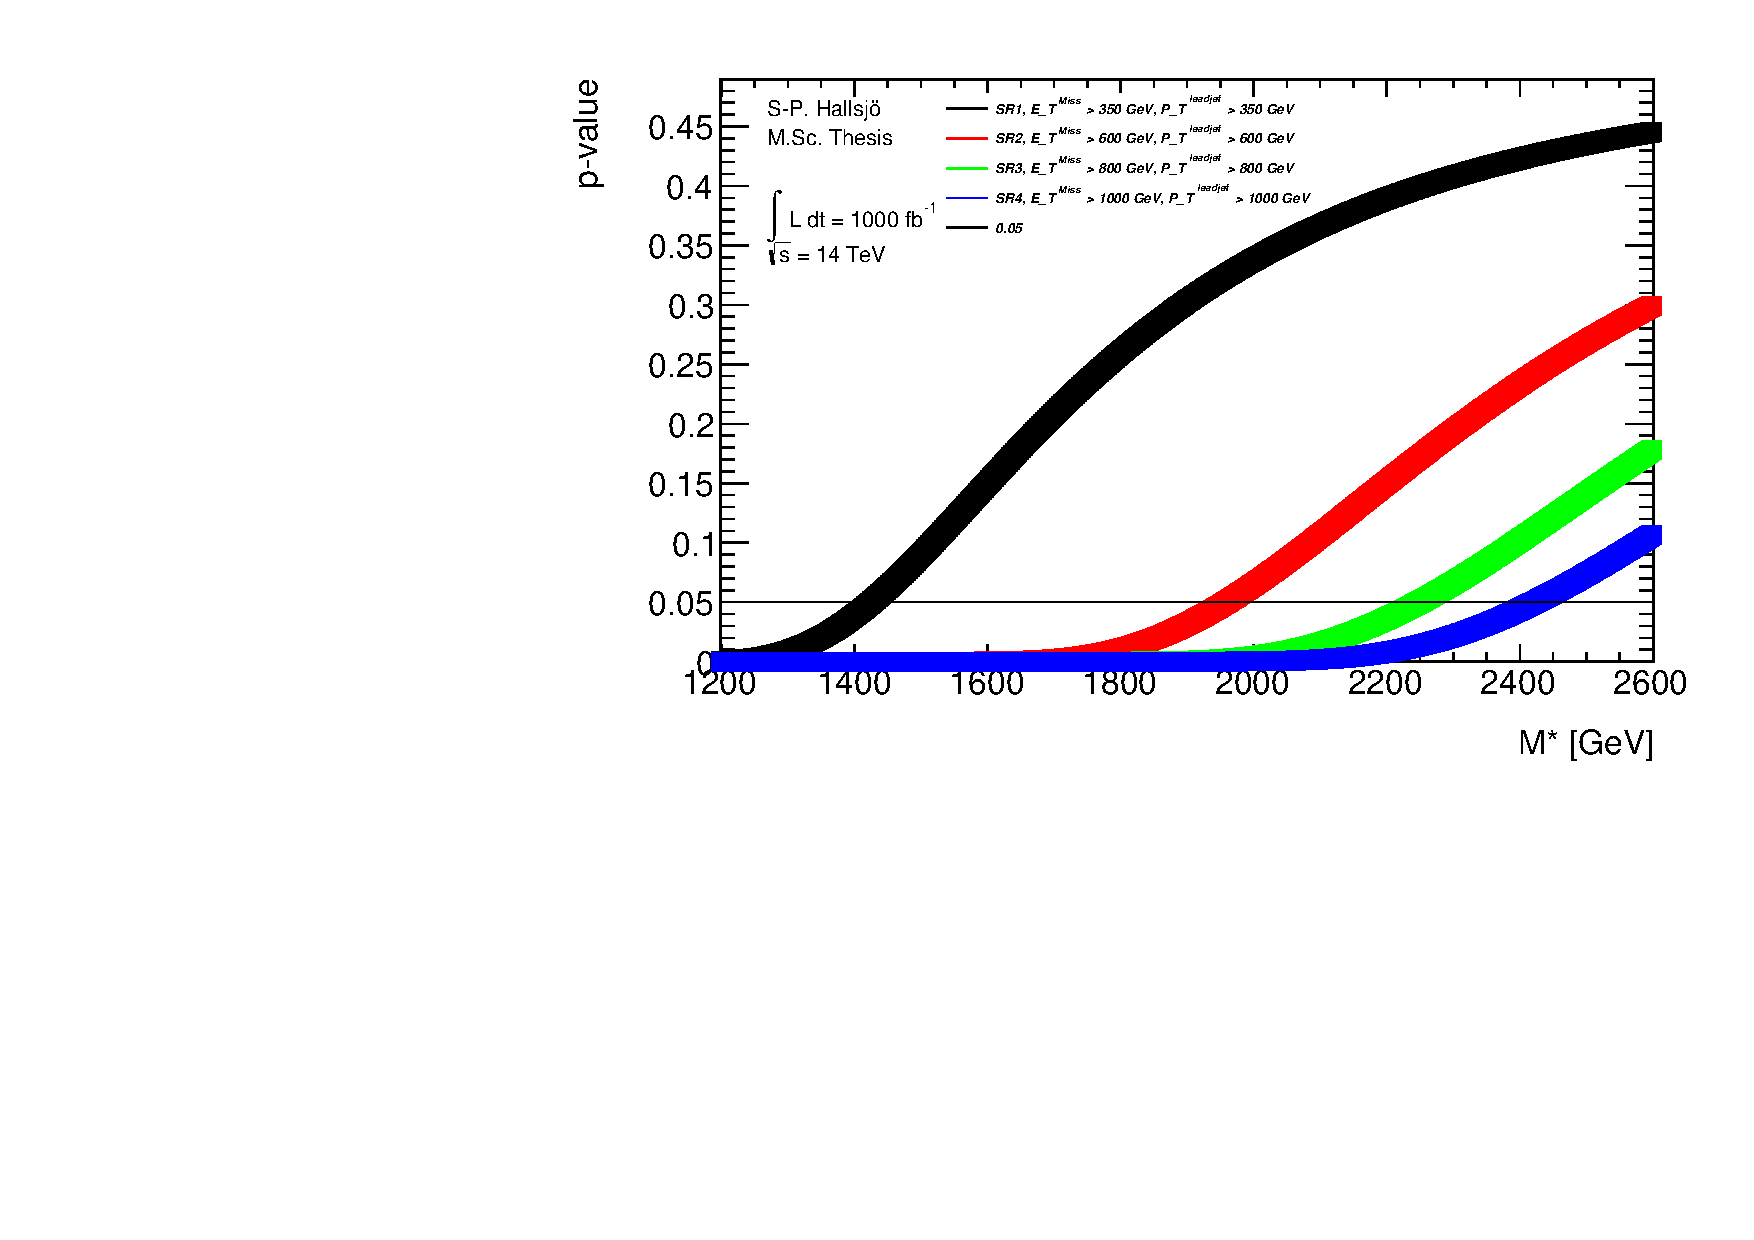
\includegraphics[width=0.5\textwidth]{Truth11.pdf}
    }
    \hfill
    \subfloat[ \label{fig:SRnewMt:2}]{%
      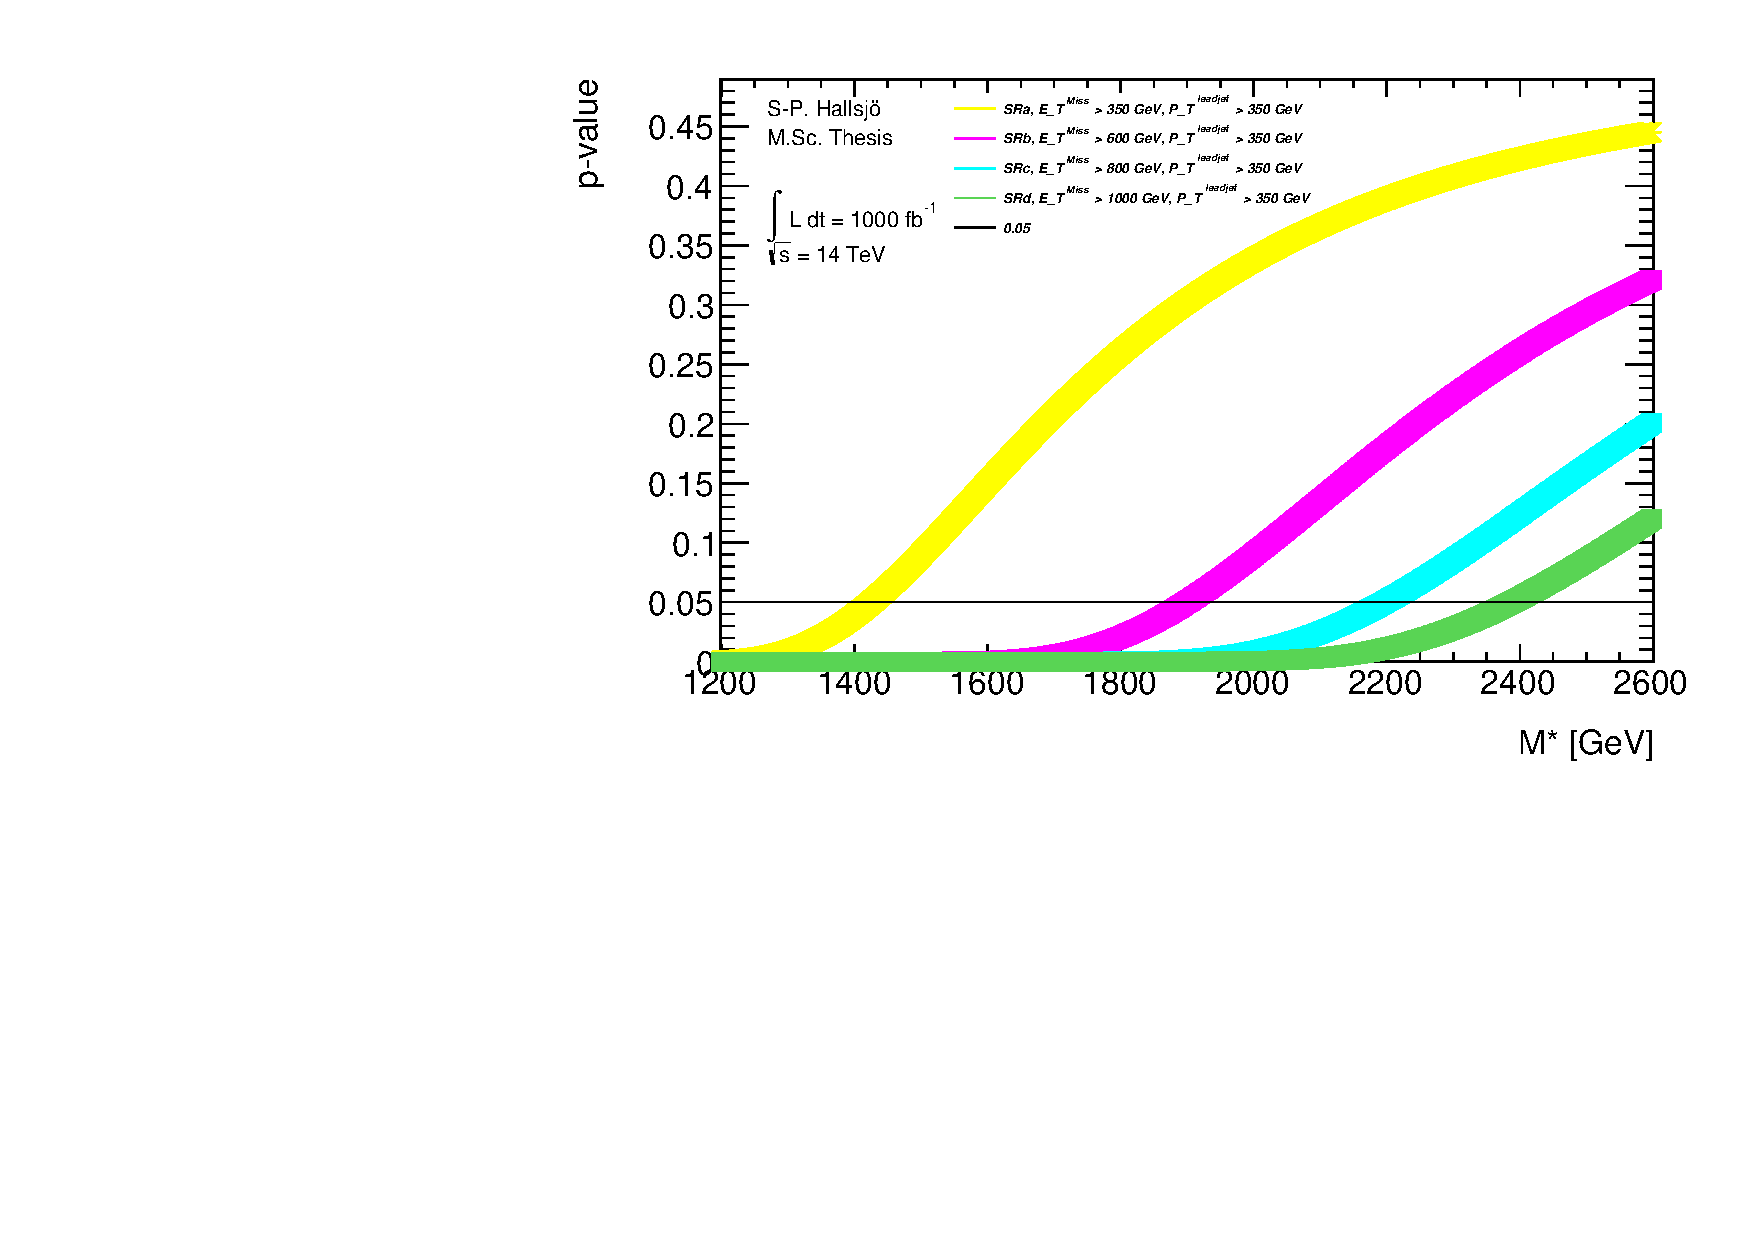
\includegraphics[width=0.5\textwidth]{Truth21.pdf}
    }
    \caption{On a truth level error model 0.02.}
    \label{fig:SRnewMt}
  \end{figure}

 \begin{figure}[H] %!ht
    \subfloat[ \label{fig:SRnewMr:1}]{%
     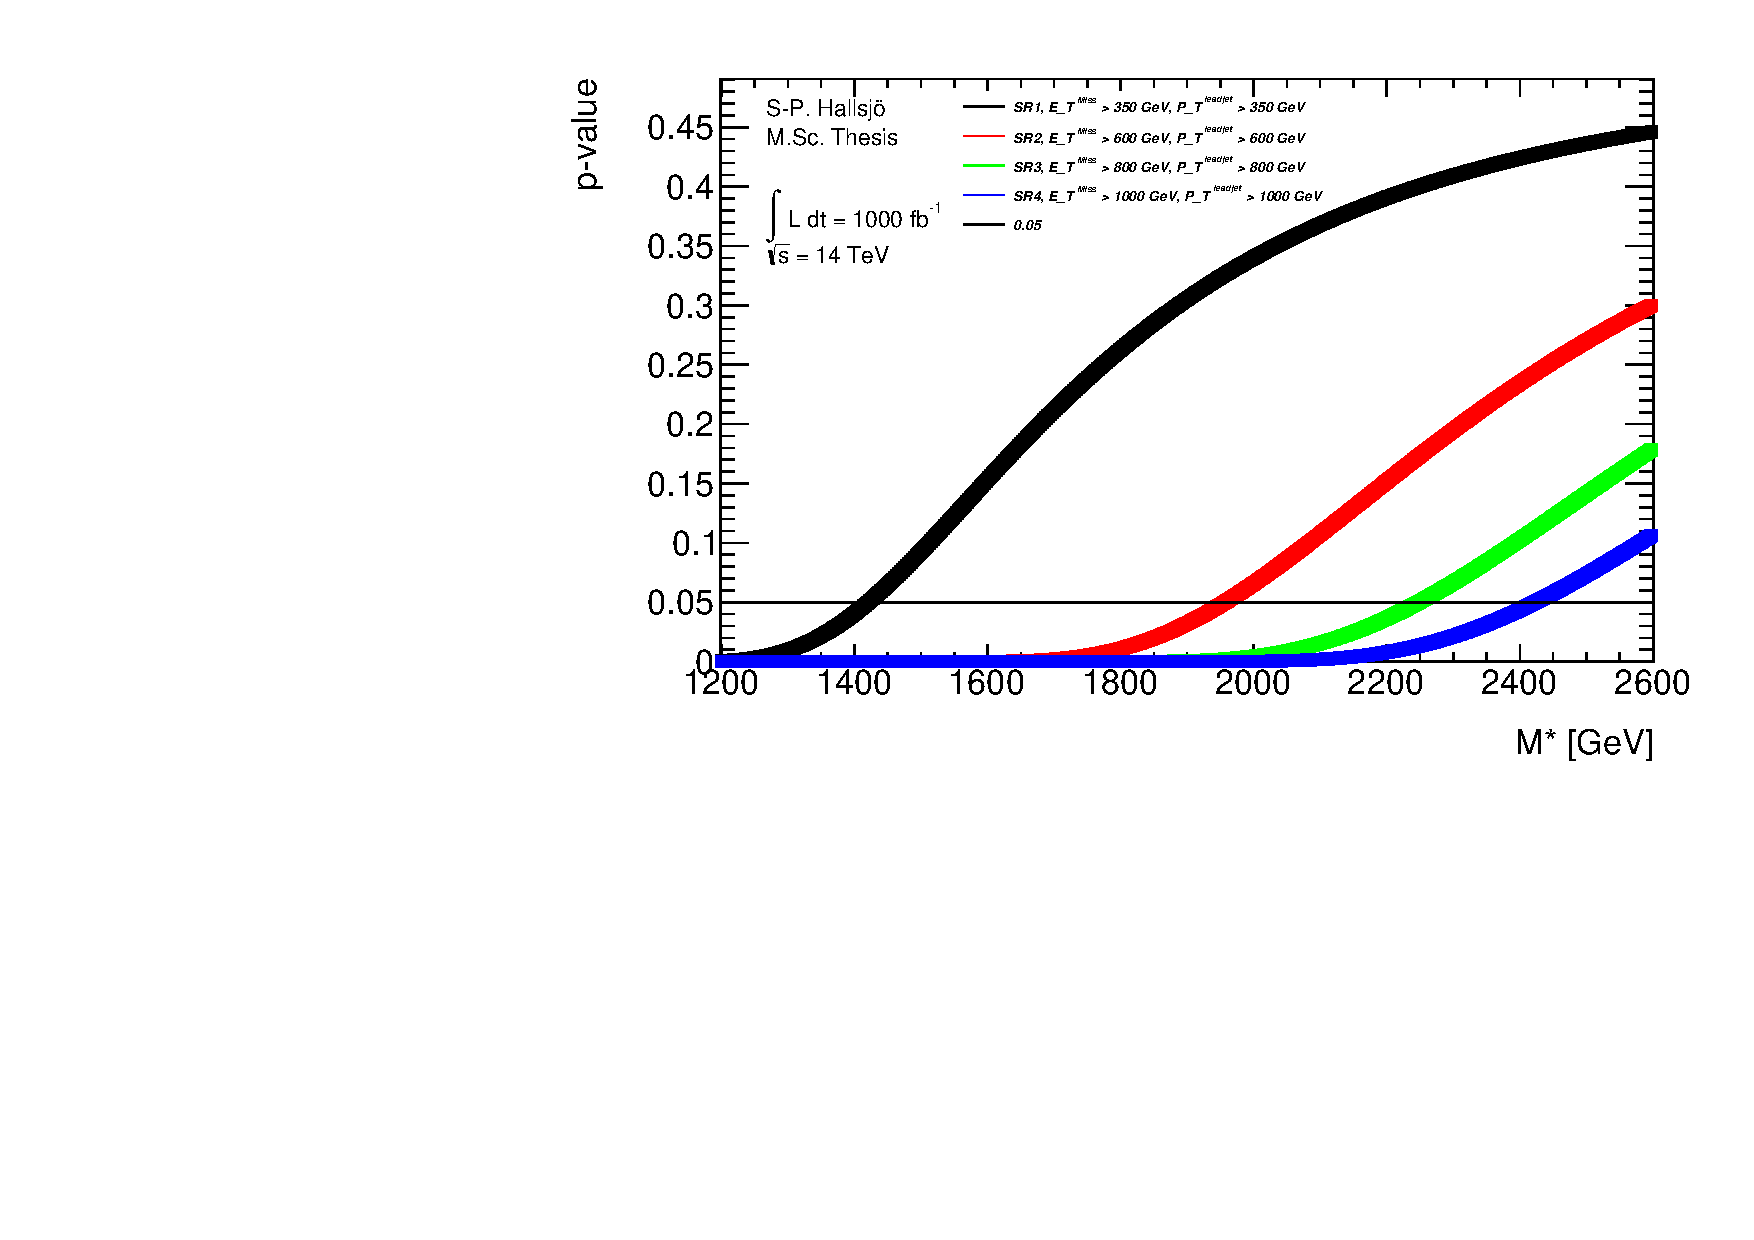
\includegraphics[width=0.5\textwidth]{Reco11.pdf}
    }
    \hfill
    \subfloat[ \label{fig:SRnewMr:2}]{%
      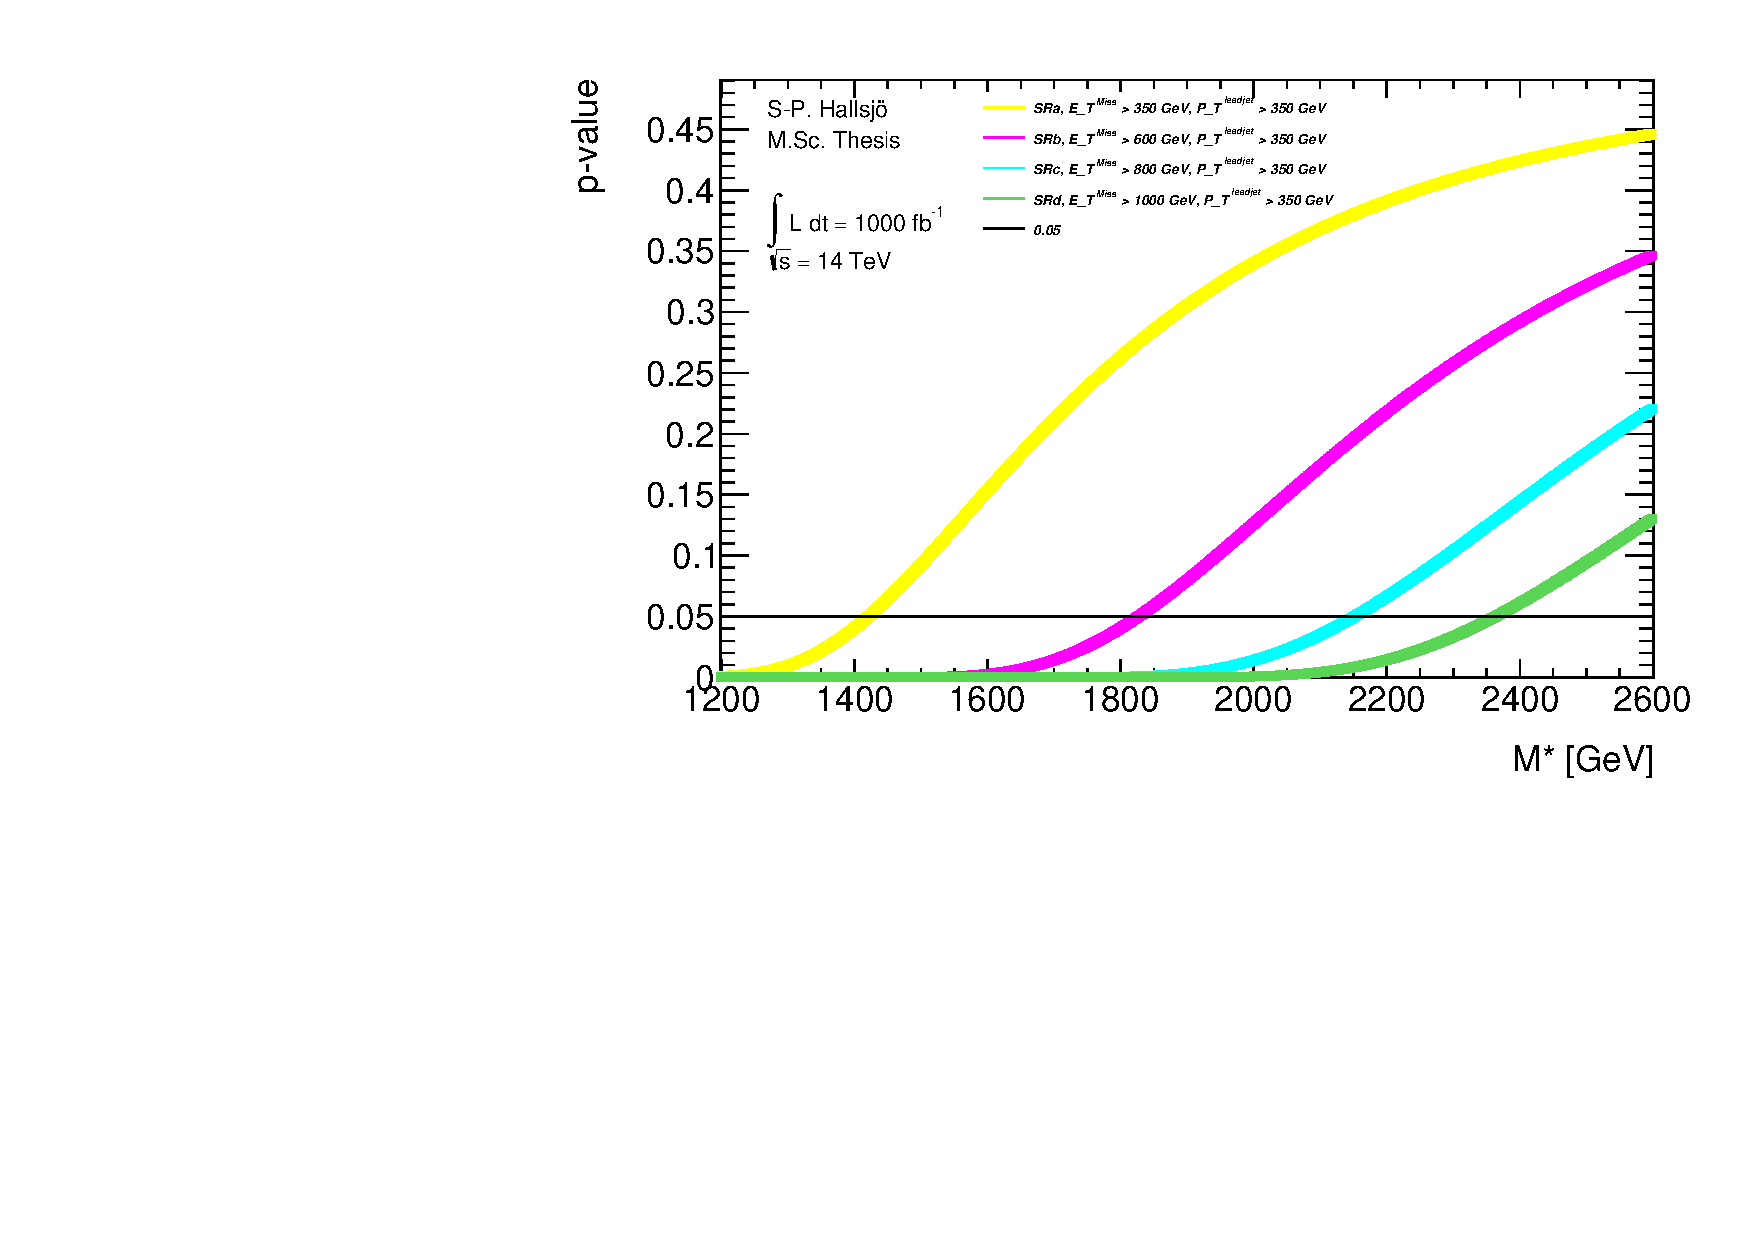
\includegraphics[width=0.5\textwidth]{Reco21.pdf}
    }
    \caption{On a reco level error model 0.02.}
    \label{fig:SRnewMr}
  \end{figure}


\begin{table}[ht]
\begin{center}
\begin{tabular}{|l|l|l|}
\hline
Signal region & Mass suppression scale Truth data & Reco data \\ \hline
SR1&1425&1420\\
SR2&1960&1957\\
SR3&2249&2248\\
SR4&2423&2423\\ \hline
SRa&1425&1421\\
SRb&1900&1827\\
SRc&2197&2152\\
SRd&2389&2363\\ \hline
\end{tabular}
\caption{Mass suppression scales in GeV given for the 0.02 error model.}
\label{tab:masssupp002}
\end{center}
\end{table}

 \begin{figure}[H] %!ht
    \subfloat[ \label{fig:SRnewM2t:1}]{%
     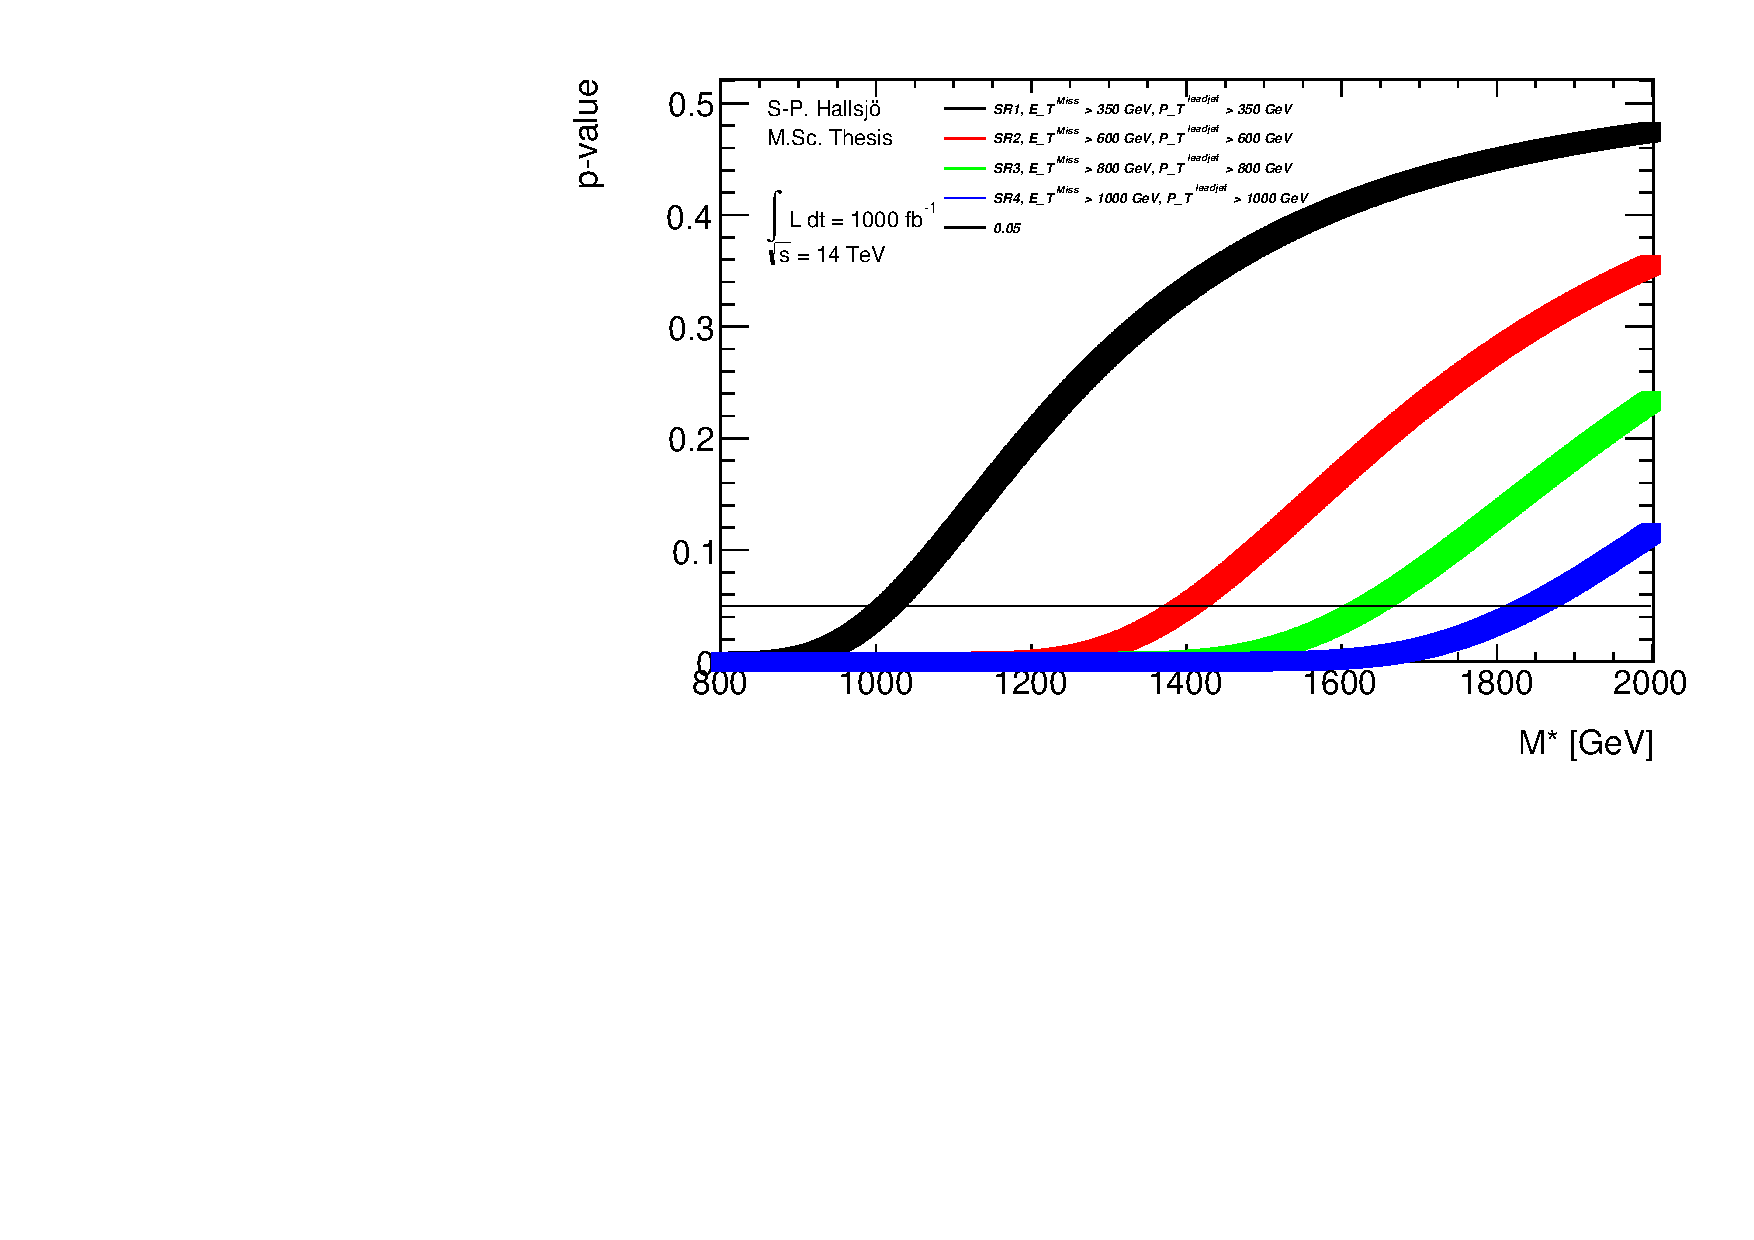
\includegraphics[width=0.5\textwidth]{Truth12.pdf}
    }
    \hfill
    \subfloat[ \label{fig:SRnewM2t:2}]{%
      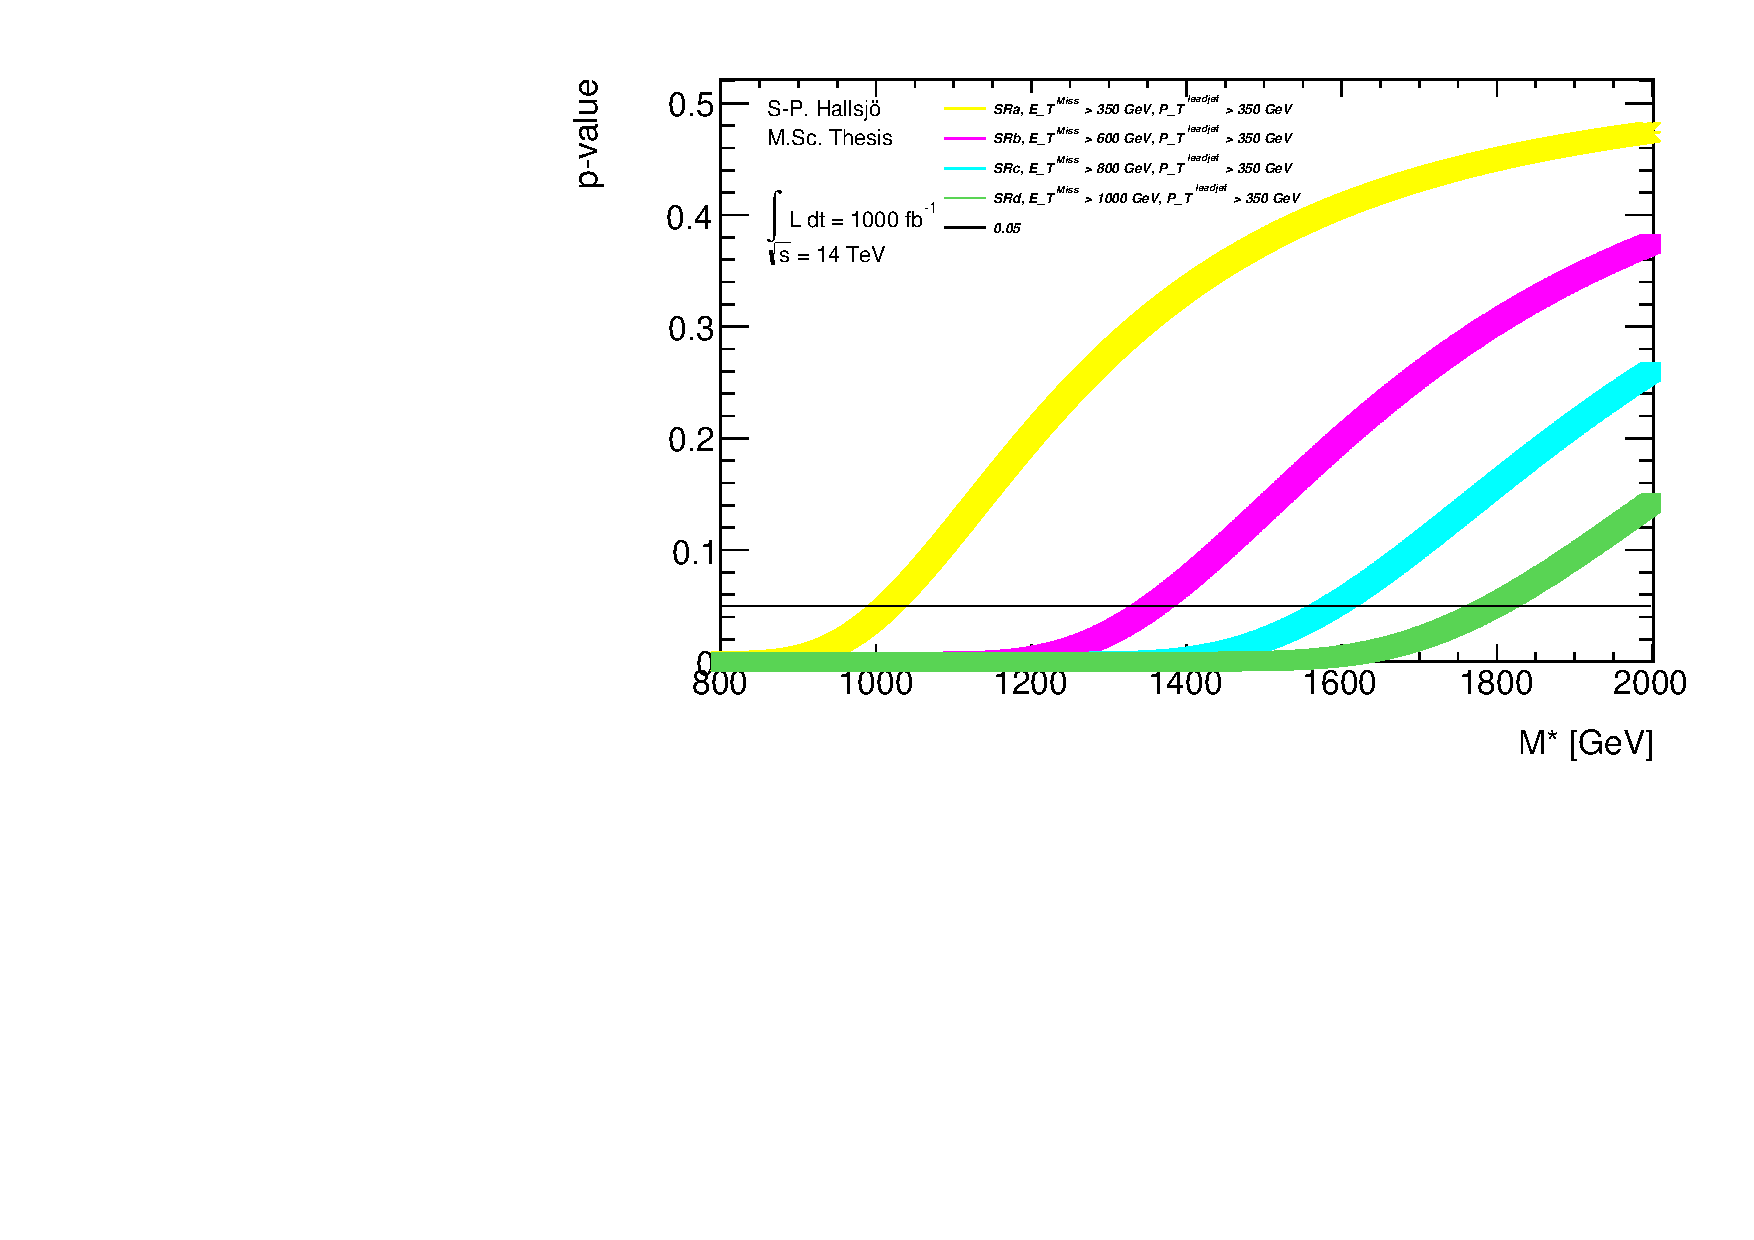
\includegraphics[width=0.5\textwidth]{Truth22.pdf}
    }
    \caption{On a truth level error model 0.10.}
    \label{fig:SRnewM2t}
  \end{figure}

 \begin{figure}[H] %!ht
    \subfloat[ \label{fig:SRnewM2r:1}]{%
     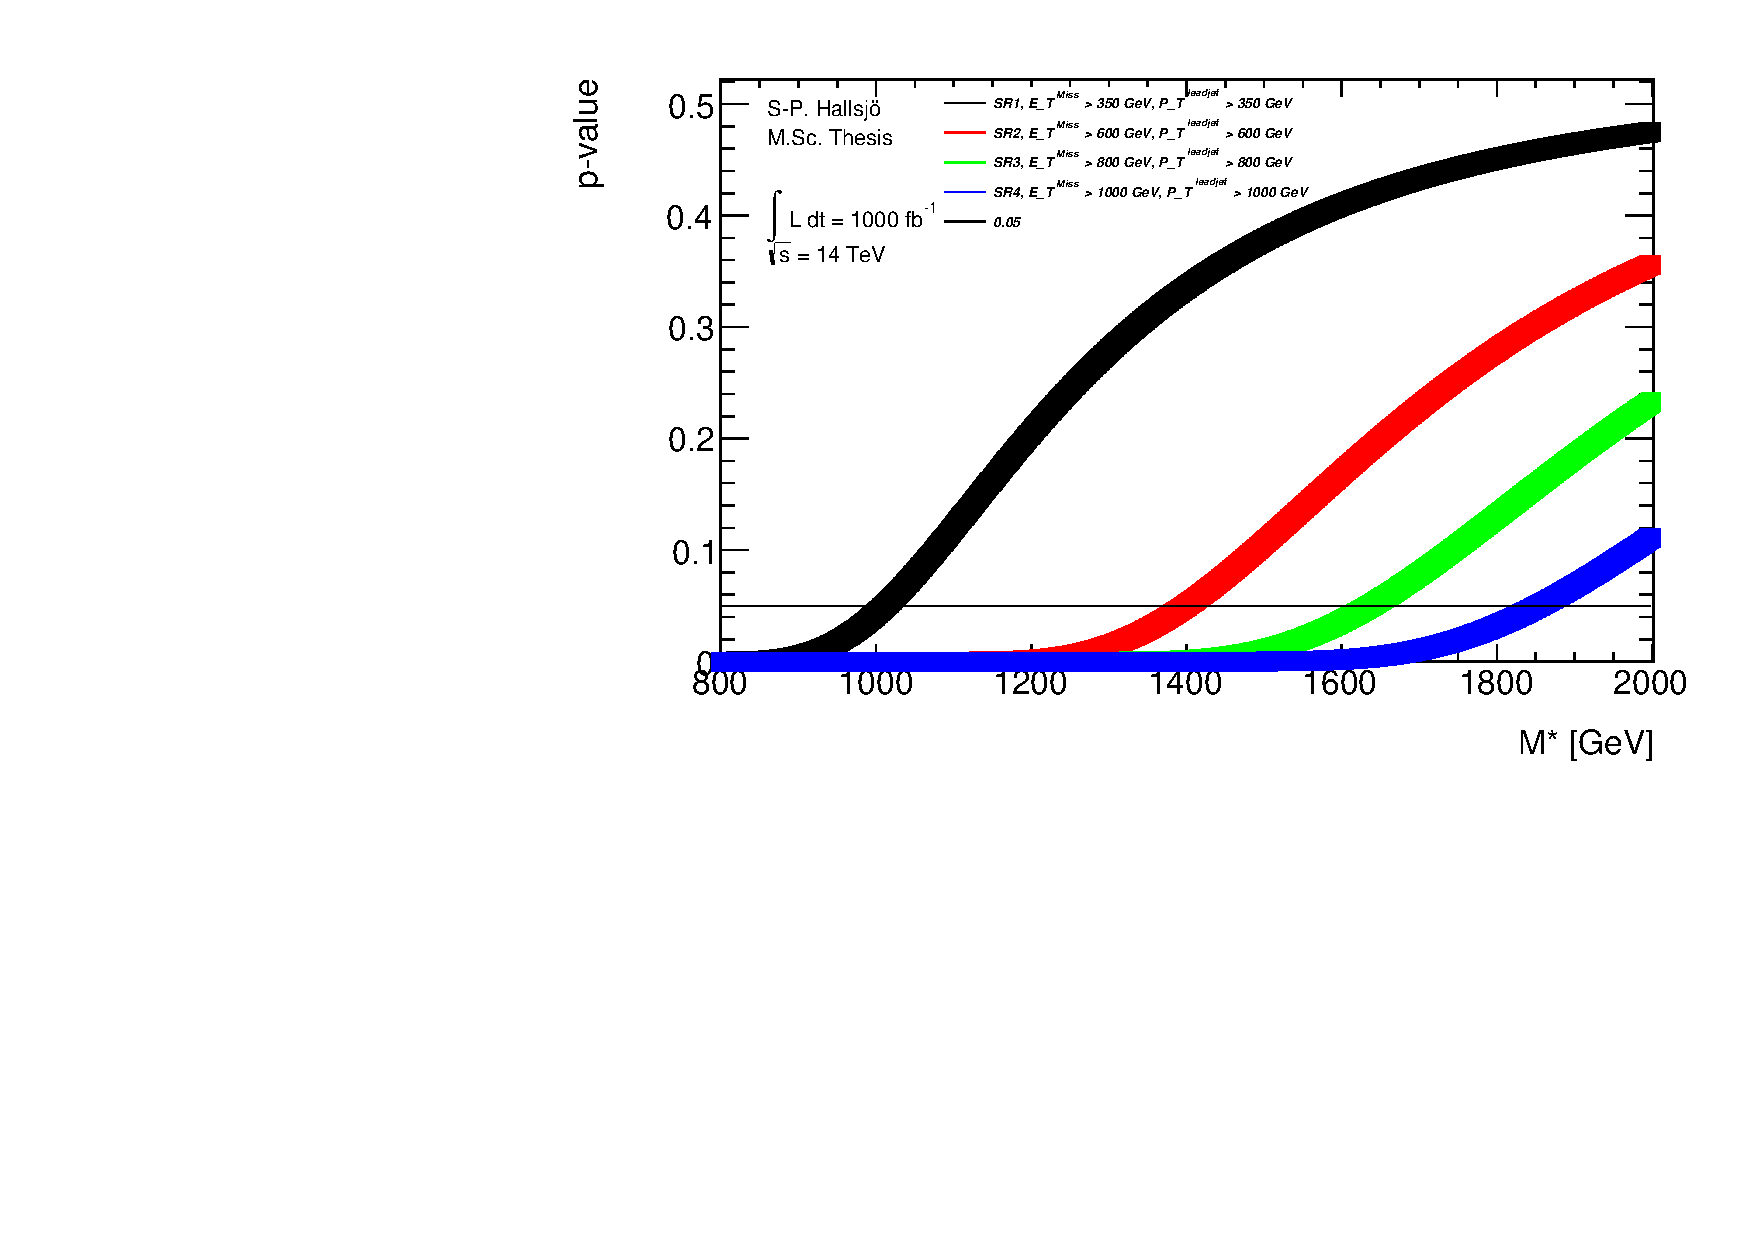
\includegraphics[width=0.5\textwidth]{Reco12.pdf}
    }
    \hfill
    \subfloat[ \label{fig:SRnewM2r:2}]{%
      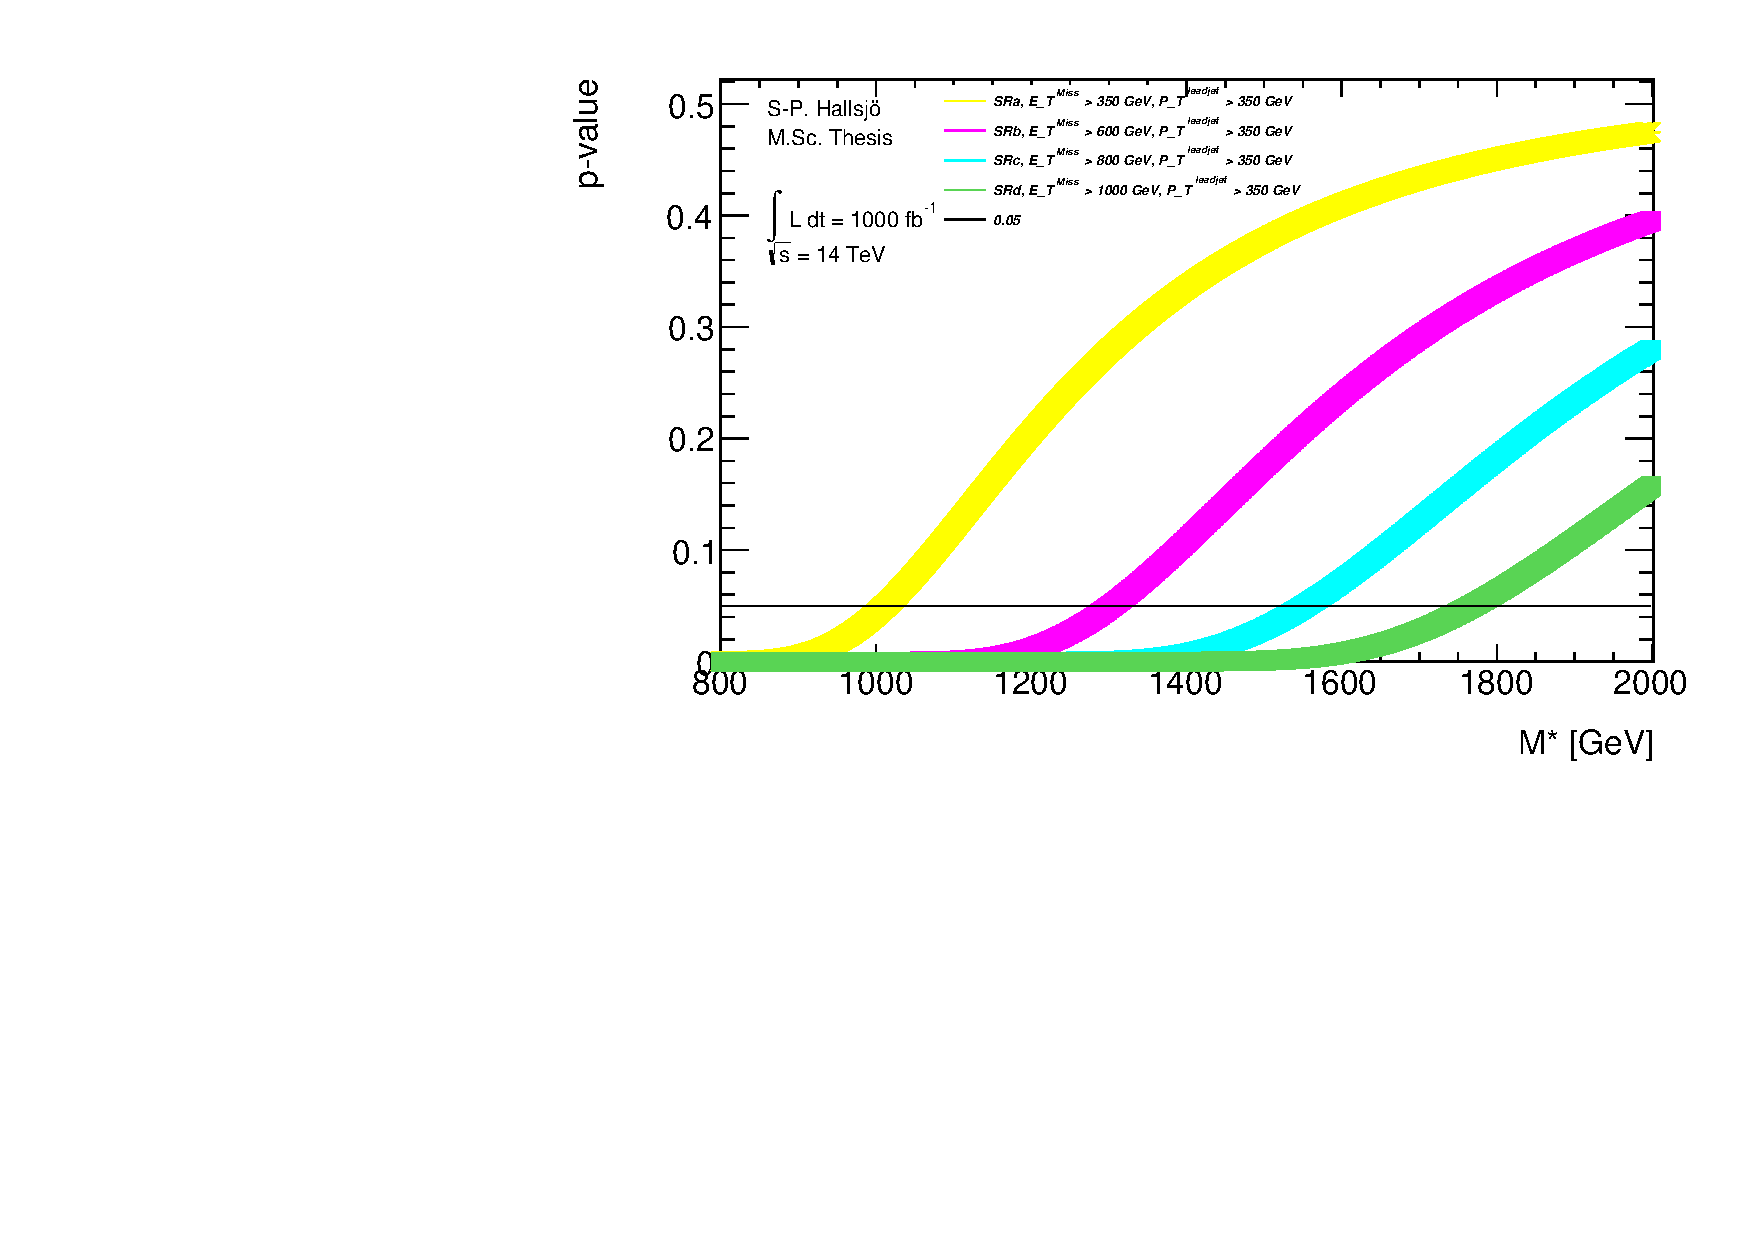
\includegraphics[width=0.5\textwidth]{Reco22.pdf}
    }
    \caption{On a reco level error model 0.10.}
    \label{fig:SRnewM2r}
  \end{figure}

\begin{table}[ht]
\begin{center}
\begin{tabular}{|l|l|l|}
\hline
Signal region & Mass suppression scale Truth data & Reco data \\ \hline
SR1&1015&1012\\
SR2&1400&1400\\
SR3&1636&1637\\
SR4&1846&1854\\ \hline
SRa&1015&1012\\
SRb&1356&1303\\
SRc&1589&1553\\
SRd&1796&1768\\ \hline
\end{tabular}
\caption{Mass suppression scales in GeV given for the 0.10 error model.}
\label{tab:masssupp010}
\end{center}
\end{table}

\subsection{Effect of pile-up on M*}
Hardly any effect. 10 \% or in that vicinity.

\subsection{Previous results}
10fb paper.
Preliminary not that much better results for 1000fb-1 and 14TeV.

The whole discussion with Steven and David.


\subsection{Limit on mediator mass}\label{sec:res:subsec:Mm}
Are there previous results?
Signal vs background plot in normal and log scale for one of the vector mediator models, to be able to evaluate all the different models the so called p-value was used in different signal regions. Below are two figures showing one of the vector mediator models in SR3.
 \begin{figure}[H] %!ht
    \subfloat[Signal on background plot for E$^{Miss}_T$ on reco level in SR3. \label{fig:sigback:1}]{%
     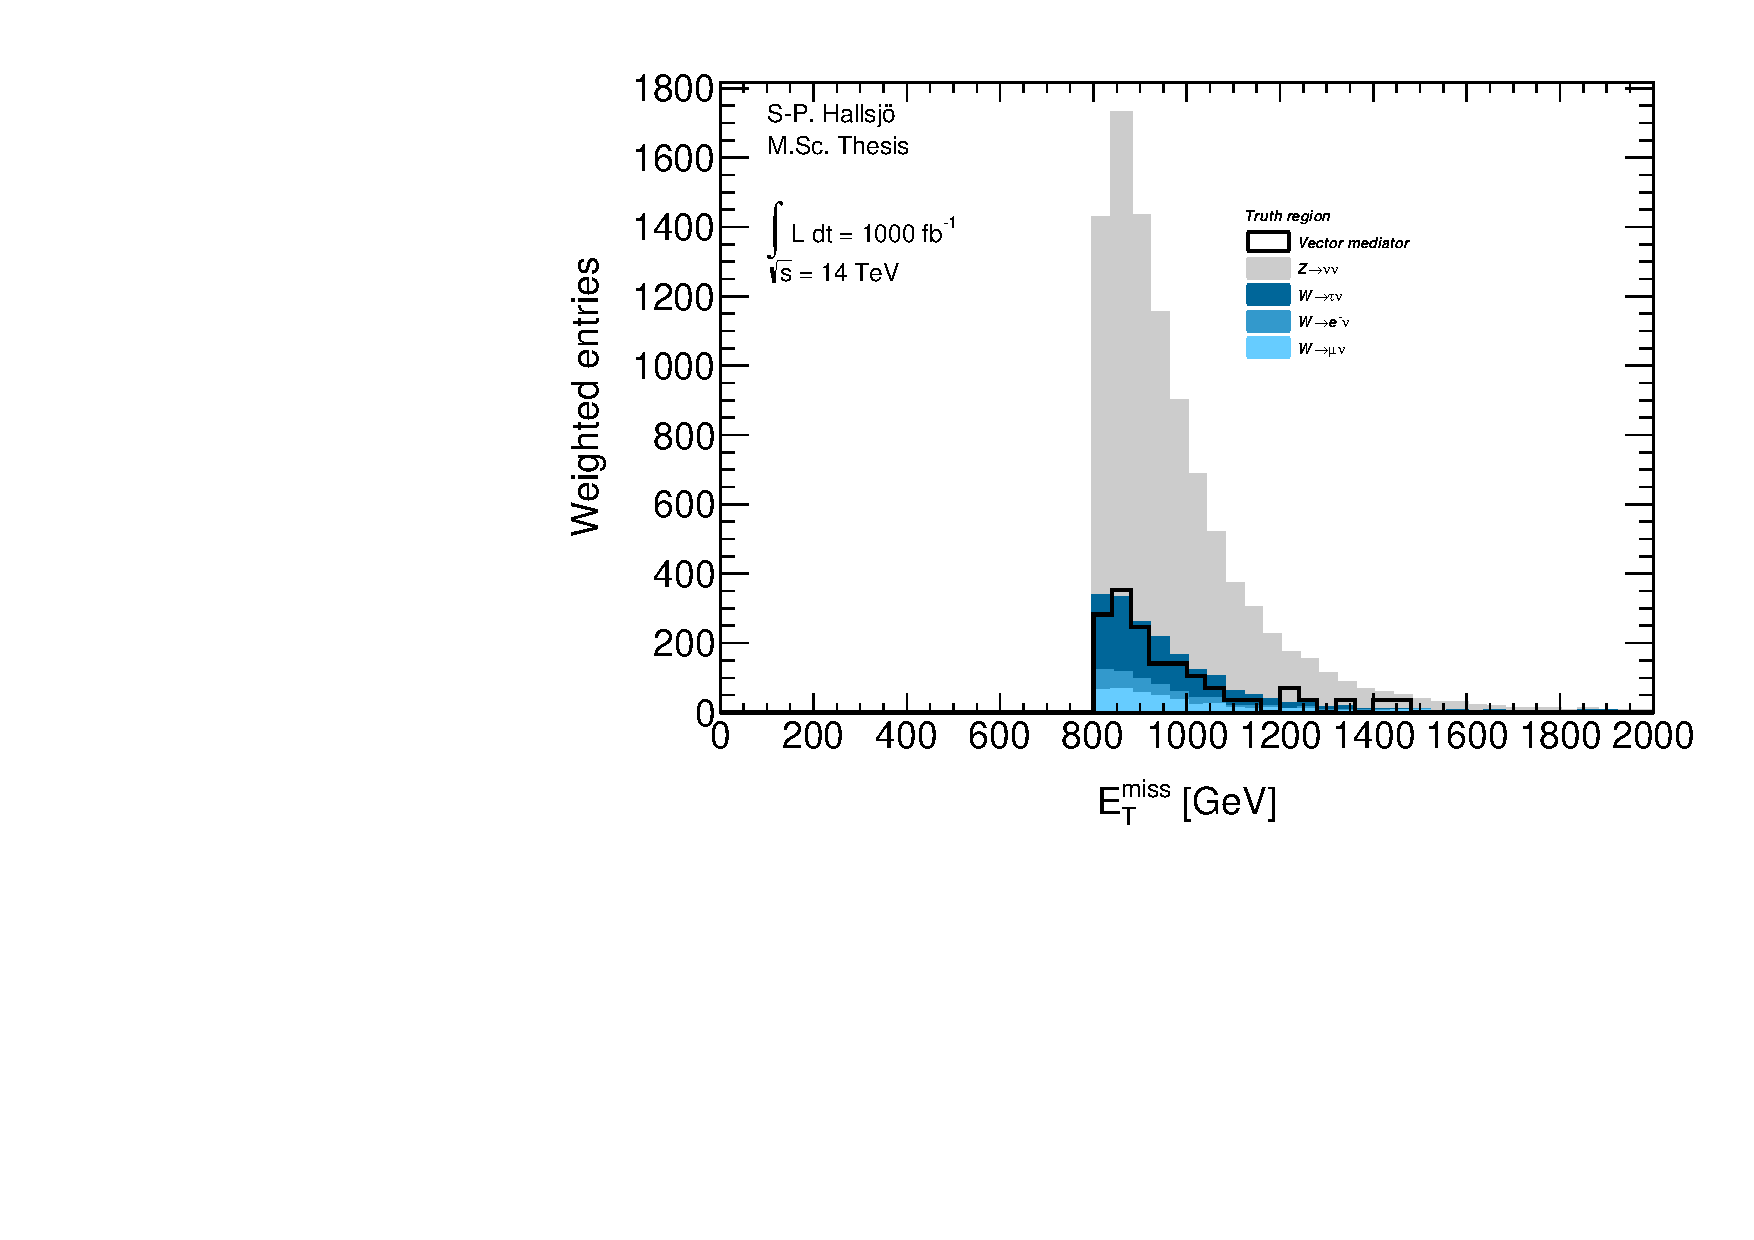
\includegraphics[width=0.5\textwidth]{exsig2sr3.pdf}
    }
    \hfill
    \subfloat[The same as a) with log scale on the y-axis \label{fig:sigbacktau:2}]{%
      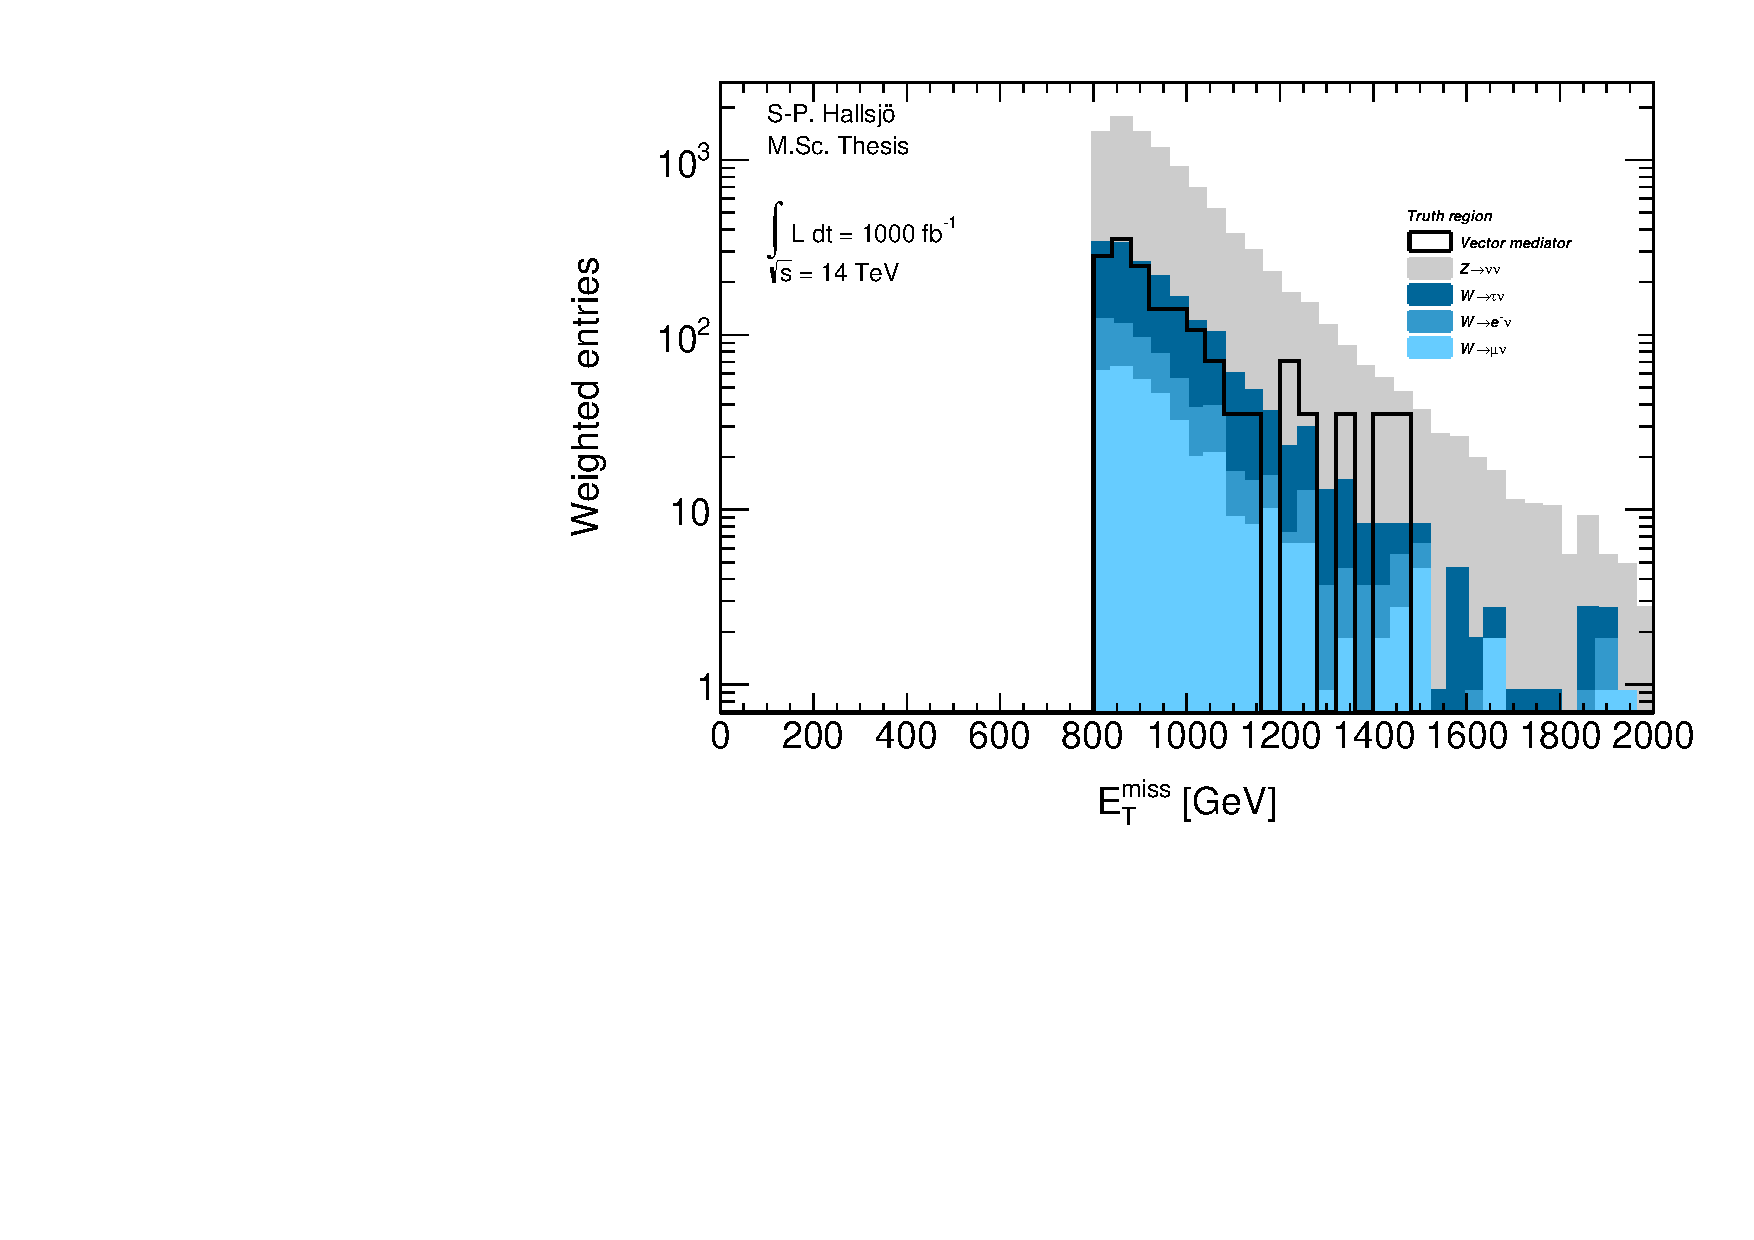
\includegraphics[width=0.5\textwidth]{exsig2sr3log.pdf}
    }
    \caption{Signal on background plot to illustrate the a general plot. }
    \label{fig:sigback}
  \end{figure}

To set a limit on the mediator mass the p-value was calculated in different signal regions for the different signal models with different mediator mass. This resulted in the following plot:


\subsection{Effect of pile-up on mediator mass}
Check the different cases for reco and truth to see what happens.
\newpage
\section{Discussion}
\subsection{Comparison to previous results}
\subsection{Effect of the high luminosity}
\newpage
\section{Conclusion}
\subsection{Limit on M*}
\subsection{Limit on mediator mass}